\documentclass[xcolor=dvipsname, handout]{beamer} %handout, ignorenonframetext

%\usepackage[ngerman]{babel}
\usepackage[utf8]{inputenc}
\usepackage{amsmath}
\usepackage{graphicx}
\usepackage{subfigure}
\usepackage{multimedia}
\usepackage{wrapfig}
\usepackage{listings}
\usepackage{comment}
\usepackage{framed,color}
\usepackage{listings}


\fboxsep=1pt%padding thickness
\fboxrule=1pt%border thickness
\usepackage{fancybox}

\usepackage{lipsum}
\usepackage{tabularx}
\usepackage{colortbl}
\usepackage{url}


\hypersetup{
	linkcolor=DarkSkyBlue,
	citecolor= DarkSkyBlue,
	filecolor= DarkSkyBlue,
	urlcolor= DarkSkyBlue
}


% COLOR-DEFINITION
%%%%%%%%%%%%%%%%%%%%%%%%
\definecolor{LightButter}{rgb}{0.98,0.91,0.31}
\definecolor{LightOrange}{rgb}{0.98,0.68,0.24}
\definecolor{LightChocolate}{rgb}{0.91,0.72,0.43}
\definecolor{LightChameleon}{rgb}{0.54,0.88,0.20}
\definecolor{LightSkyBlue}{rgb}{0.45,0.62,0.81}
\definecolor{LightPlum}{rgb}{0.68,0.50,0.66}
\definecolor{LightScarletRed}{rgb}{0.93,0.16,0.16}
\definecolor{LightGray}{rgb}{0.80,0.80,0.80}
\definecolor{Butter}{rgb}{0.93,0.86,0.25}
\definecolor{Orange}{rgb}{0.96,0.47,0.00}
\definecolor{Chocolate}{rgb}{0.75,0.49,0.07}
\definecolor{Chameleon}{rgb}{0.45,0.82,0.09}
\definecolor{SkyBlue}{rgb}{0.20,0.39,0.64}
\definecolor{Plum}{rgb}{0.46,0.31,0.48}
\definecolor{ScarletRed}{rgb}{0.80,0.00,0.00}
\definecolor{DarkButter}{rgb}{0.77,0.62,0.00}
\definecolor{DarkOrange}{rgb}{0.80,0.36,0.00}
\definecolor{DarkChocolate}{rgb}{0.56,0.35,0.01}
\definecolor{DarkChameleon}{rgb}{0.30,0.60,0.02}
\definecolor{DarkSkyBlue}{rgb}{0.12,0.29,0.53}
\definecolor{DarkPlum}{rgb}{0.36,0.21,0.40}
\definecolor{DarkScarletRed}{rgb}{0.64,0.00,0.00}



% HPI-THEME
%%%%%%%%%%%%%%%%%%%%%%%%
\RequirePackage{scrlfile}
%\ReplaceFile{beamerthemehpiswa.sty}{theme/beamerthemehpiswa.sty}
%\ReplaceFile{beamercolorthemehpiswa.sty}{theme/beamercolorthemehpiswa.sty}
%\ReplaceFile{beamerfontthemehpiswa.sty}{theme/beamerfontthemehpiswa.sty}
%\ReplaceFile{beamerinnerthemehpiswa.sty}{theme/beamerinnerthemehpiswa.sty}
%\ReplaceFile{beamerouterthemehpiswa.sty}{theme/beamerouterthemehpiswa.sty}
%\ReplaceFile{hpi.png}{theme/hpi.png}
\usetheme{hpiswa}


% BEAMER-Anpassungen
%%%%%%%%%%%%%%%%%%%%%%%%
\setbeamercolor{block title}{bg=DarkOrange}
\setbeamercolor{block body}{bg=Orange!20}
%\setbeamercolor{block title alerted}{bg=red}
\setbeamercolor{block body alerted}{bg=red!20}
%\setbeamercolor{block title example}{bg=green}
\setbeamercolor{block body example}{bg=DarkChameleon!20}
%\usecolortheme[RGB={205,173,0}]{structure}
\usecolortheme[RGB={30,74,135}]{structure}

\usecolortheme{orchid}
%\usefonttheme{professionalfonts}
%\useoutertheme[subsection=false]{smoothbars}
%\useinnertheme{rectangles}
%\setbeamertemplate{blocks}[shadow=true]

\setbeamercovered{transparent}
\setbeamertemplate{navigation symbols}{}%remove navigation symbols



% Eigene Anpassungen
%%%%%%%%%%%%%%%%%%%%

% Explainframes:
\usepackage{ifthen}
\newboolean{isexplainframe}
\setboolean{isexplainframe}{false}
\mode<handout>{
\newenvironment{explainframe}[1]{
\setboolean{isexplainframe}{true}
\addtocounter{framenumber}{-1}
\setbeamertemplate{background}[grid][step=5mm,color=LightGray]
\begin{frame}[fragile,environment=explainframe]{Handout only: #1}%
}{%
\end{frame}%
\setboolean{isexplainframe}{false}
}}
\mode<beamer>{
\excludecomment{explainframe}
}

\setbeamertemplate{footline}{%
	\leavevmode%
	\hbox{%
		\begin{beamercolorbox}[wd=.45\paperwidth,ht=2.25ex,dp=1ex,center]{author in head/foot}%
			\usebeamerfont{author in head/foot}\insertinstitute
		\end{beamercolorbox}%
		\begin{beamercolorbox}[wd=.2\paperwidth,ht=2.25ex,dp=1ex,center]{title in head/foot}%
			\usebeamerfont{title in head/foot}\insertshorttitle
		\end{beamercolorbox}%
		\begin{beamercolorbox}[wd=.35\paperwidth,ht=2.25ex,dp=1ex,right]{date in head/foot}%
			\usebeamerfont{date in head/foot}\insertshortdate{}\hspace*{2em}
			\insertframenumber{}\ifthenelse{\boolean{isexplainframe}}{E}{} / \inserttotalframenumber\hspace*{2ex}
	\end{beamercolorbox}}%
	\vskip0pt%
}

\definecolor{javared}{rgb}{0.6,0,0} % for strings
\definecolor{javagreen}{rgb}{0.25,0.5,0.35} % comments
\definecolor{javapurple}{rgb}{0.5,0,0.35} % keywords
\definecolor{javadocblue}{rgb}{0.25,0.35,0.75} % javadoc

\lstset{
  language=Ruby,
  basicstyle=\scriptsize\ttfamily,
  keywordstyle=\color{javapurple}\bfseries,
  stringstyle=\color{javared},
  commentstyle=\color{javagreen},
  morecomment=[s][\color{javadocblue}]{/**}{*/},
  tabsize=4,
  showspaces=false,
  showstringspaces=false,
  breaklines=true
}


% Gliederung vor jedem Punkt:
\AtBeginSection[]{
\ifthenelse{\equal{\value{section}}{1}}{}{
\ifthenelse{\equal{\value{section}}{6}}{}{
\begin{frame}{Overview}
	\tableofcontents[currentsection, hideothersubsections]
\end{frame}
}
}
}


% Quote-Environment:

\renewenvironment{quote}{%
\begin{exampleblock}{}%
\begin{center}%
\begin{large}%
``}{%
''\end{large}%
\end{center}%
\end{exampleblock}}




% Dokument-Meta-Daten:
%%%%%%%%%%%%%%%%%%%%%%%
\title{BETA and Newspeak}
\subtitle{Seminar Module Systems, SS2015}
\author{Fabio Niephaus, Matthias Springer}
\date{\today}
\institute[2012]{Hasso Plattner Institute, Software Architecture Group}



\begin{document}

\begin{frame}[plain]
	\maketitle
\end{frame}
\begin{frame}{Overview}
	\tableofcontents[hideallsubsections]
\end{frame}


\section{Introduction}
%%%%%%%%%%%%%%%
%%%%%%%%%%%%%%%

\begin{frame}{Introduction}
\begin{itemize}
    \item BETA: ``A modern language in the Simula tradition''
    \begin{itemize}
      \item Designed by Birger Møller-Pedersen and Kristen Nygaard (\emph{Scandinavian School})
      \item Class = Method = Pattern
      \item Nested Patterns
    \end{itemize}
    \item Newspeak: ``A new programming language in the tradition of Self and Smalltalk''
    \begin{itemize}
      \item Designed by Gilad Bracha et al.
      \item Nested Classes
      \item No globals: all names are late bound
    \end{itemize}
\end{itemize}
\end{frame}

\section{Unification: The Pattern}

\begin{frame}[fragile]{Patterns}
\begin{itemize}
  \item Classes and methods are patterns
  \item ``Patterns [are] templates for generating objects (instances).''
  \item Objects are executable
\end{itemize}
\vfill
\begin{verbatim}
Pattern: (# 
  Declaration1; Declaration2; ...; DeclarationN
  enter InputArguments
  do Implementation
  exit OutputArguments
#)
\end{verbatim}
\end{frame}

\begin{frame}{Unification of Abstraction Mechanisms: The Pattern\textsuperscript{[7]}}
\begin{itemize}
\item Instances of a procedure are procedure activations
\item Instances of a class are objects
\item Instances of a function are function activations
\item Instances of a type are values
\end{itemize}
\end{frame}

\begin{explainframe}{Similarities between Objects and Procedure Activations}
\begin{itemize}
  \item Procedure activation = Activation record + execution of code
  \item Activation record is similar to object: data items and local procedures (nested procedures in languages with block structure)
\end{itemize}
\end{explainframe}

\begin{frame}[fragile]{Example}
\begin{verbatim}
(# 
    Account: (#  balance: @integer;
        Deposit:
          (# amount: @integer
             enter amount
             do balance+amount->balance
             exit balance
          #);
        Withdraw: (# ... #);
    #);
   account: @Account;
   K1: @integer;
   do 
     100->&account.Deposit;
     50->&account.Withdraw->K1;
#)
\end{verbatim}
\end{frame}

\begin{explainframe}{Beta Syntax}
\begin{itemize}
  \item \texttt{(\# ... \#)} for block structure
  \item \texttt{$@$Type} for static references
  \item \texttt{\^{}Type} for dynamic references
  \item \texttt{\&Type} for instance creation
  \item \texttt{[]} aquires a references instead of object execution
  \item \texttt{\&Account[]} returns a dynamic reference to a new account instance
\end{itemize}
\end{explainframe}

\begin{frame}{Subpatterns}{Specialization by Simple Inheritance}
\begin{align*} 
  Resulting \ properties &= & inherited \ properties &+ new \ properties\\
  Resulting \ behavior &= & inherited \ behavivor &+ new \ behavior\\
  Resulting \ arguments &= & inherited \ arguments &+ new \ arguments\\
  Resulting \ results &= & inherited \ results &+ new \ results
\end{align*}
\begin{itemize}
  \item Method execution starts at base method: use \texttt{inner} to call specialized method
\end{itemize}
\end{frame}

\begin{explainframe}{Virtual Patterns and Pattern Variables}
  \begin{itemize}
    \item Non-virtual pattern: entire type hierarchy has same pattern
    \item Virtual pattern: subtypes can have different patterns
    \item Pattern variables: every object can have a different pattern
  \end{itemize}
\end{explainframe}

\begin{frame}{Pattern (Design) Patterns}
  \begin{itemize}
    \item \textbf{Procedure Pattern}: sequence of actions
    \item \textbf{Function Pattern}: sequence of actions with return value(s), does not change state
    \item \textbf{Class Pattern}: template for generating objects
  \end{itemize}
\end{frame}

\begin{frame}{Expected Benefits of Unification\textsuperscript{[6]}}
\begin{itemize}
  \item Design goals \begin{itemize}
    \item ``The pattern mechanism should be the ultimate abstraction mechanism, subsuming all other known abstraction mechanisms.'' 
    \item ``The unification should be more than just the union of existing mechanisms.''
    \item ``All parts of a pattern should be meaningful, no matter how the pattern is applied.''
  \end{itemize}
  \item ``Uniform treatment of all abstraction mechanisms. [...] It ensures orthogonality among class, procedure, etc.''
  \item Functionality: subpatterns, virtual patterns, nested patterns, pattern variables
\end{itemize}
\end{frame}

\section{Nested Classes}

\begin{frame}{Nested Classes}{What is it?}
\begin{itemize}
  \item Class defined inside another class
  \item Part-of relationship: nested classes belong to the enclosing class
  \item Access to enclosing class (lookup depends on programming language)
\end{itemize}
\end{frame}

\begin{frame}{Nested Classes}{Benefits}
\begin{itemize}
  \item \textbf{Namespace} for classes, avoiding name clashes
  \item Group together what belongs together: increase \textbf{understandability} and \textbf{readability}
  \item A form of \textbf{encapsulation}, promoting development towards an interfaces instead of an implementation (using visibility annotations)
  \item Support for more advanced features \\ (e.g. Class Hierarchy Inheritance)
\end{itemize}
\end{frame}

\begin{frame}{Nested Classes}{Programming Languages}
\begin{itemize}
  \item Java: nested classes are non-virtual
  \item Ruby: inner classes/modules are non-virtual
  \item \textbf{BETA, Newspeak:} nested classes are virtual and can be overridden
\end{itemize}
\end{frame}

\begin{frame}[fragile]{BETA Nested Classes}
\begin{itemize}
  \item Virtual methods can be overridden in subclasses
  \item Virtual classes can be overridden in subclasses
  \item Virtual patterns can be overridden in subclasses
\end{itemize}
\end{frame}

\begin{frame}[fragile]{Example: BETA Nested Classes}
\begin{verbatim}
Reservation: (#
  date: @Date;
  Display:< (# do date.PrintToConsole; INNER; #)
#)

TrainReservation: Reservation (#
  seat: @Seat;
  Display::< (# do seat.PrintToConsole; INNER; #)
#)

(#
  reservation: ^Reservation;
  do
    &reservation.Display
#)
\end{verbatim}
\end{frame}

\begin{explainframe}{BETA Nested Classes}
\begin{verbatim}
Reservation: (#
  date: @Date;
  DisplayReservation: (# do date.PrintToConsole; INNER; #)
  Display:< DisplayReservation
#)

TrainReservation: Reservation (#
  seat: @Seat;
  DisplayTrainReservation: DisplayReservation (# 
    do seat.PrintToConsole; #)
  Display::< DisplayTrainReservation
#)
\end{verbatim}
\end{explainframe}

\begin{explainframe}{BETA Nested Classes}
\begin{itemize}
  \item Only virtual patterns can be overridden (denoted by \lstinline{:<})
  \item Overriding pattern must be a subpattern of superpattern
  \item Pattern execution starts with base pattern (\lstinline{inner} instead of \lstinline{super})
\end{itemize}
\end{explainframe}

\begin{frame}{Example: Nested Classes in Newspeak \textsuperscript{[2]}}
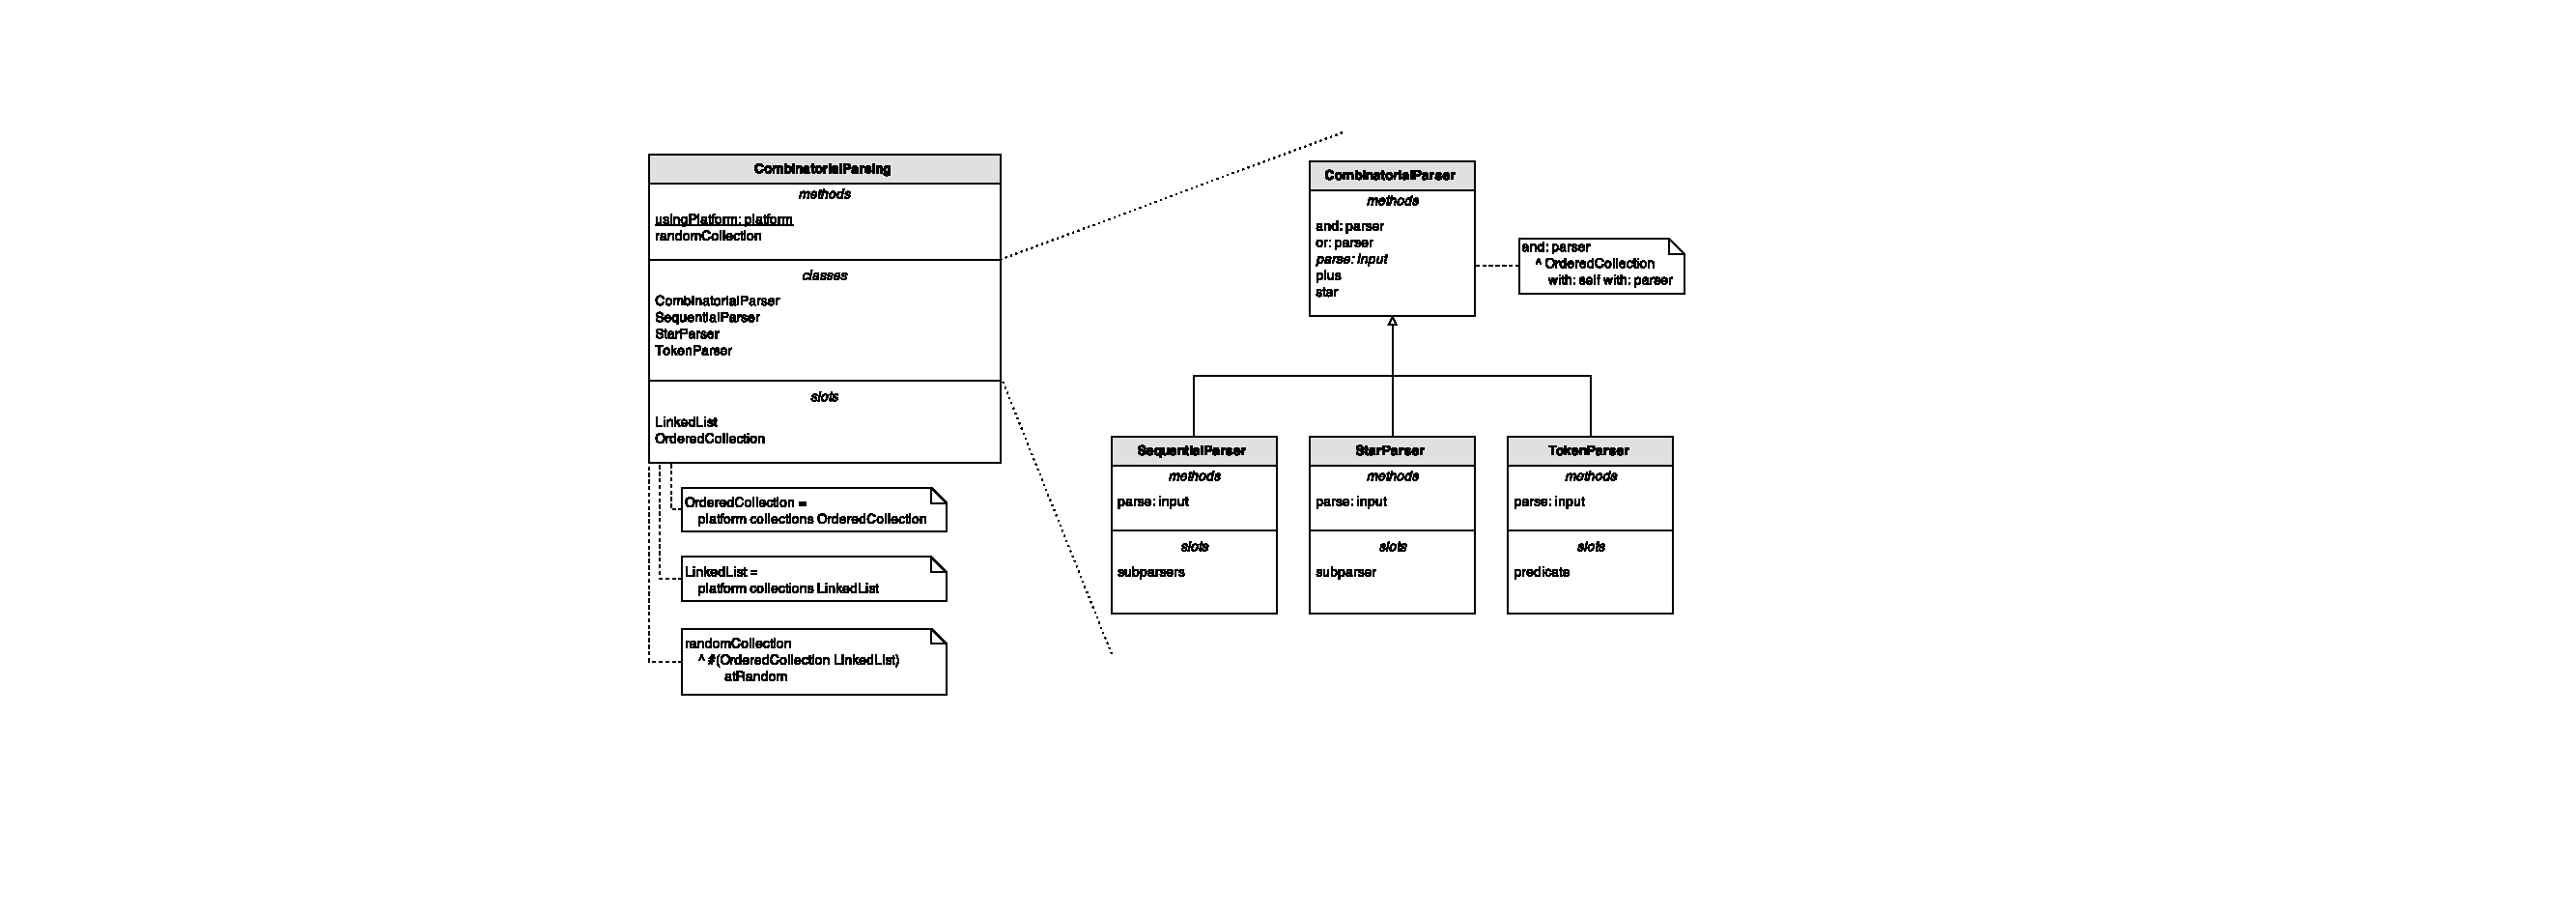
\includegraphics[width=\textwidth]{resources/newspeak_basic}
\end{frame}

\begin{explainframe}{Nested Classes in Newspeak \textsuperscript{[3]}}
\begin{itemize}
  \item \textbf{Methods:} instance methods
  \item \textbf{Classes:} nested class definitions
  \item \textbf{Slots:} instance variables
  \item \textbf{Module Definition:} a class object that acts as a module
  \begin{itemize}
    \item has to be a top-level class
    \item has its own namespace which is represented by a \lstinline{platform} object
    \item is stateless
    \item its external dependencies are listed at the top of the class
  \end{itemize}
  \item \textbf{Module:} an instance of a module definition
\end{itemize}
\end{explainframe}

\begin{frame}{\texttt{platform} Object instead of Global Namespace\textsuperscript{[8]}}
\begin{itemize}
  \item \lstinline{platform} contains references to top-level modules required by the application (mapping identifiers to top-level modules)
  \begin{itemize}
    \item Provided by the system: collections, file system, drawing, kernel classes, \ldots
    \item Provided by the developer: custom libraries
    \item Contains all dependencies required for deployment
  \end{itemize}
  \item Created using IDE support, then object graph serialization
  \item \lstinline{Platform>>main:args:} is the application's entry point
  \item \lstinline{platform} is similar to Squeak environments
\end{itemize}
\end{frame}

\begin{frame}[fragile]{Instance Creation in Newspeak}{Nested Classes in a Nutshell for Smalltalkers}
\begin{enumerate}
  \item Message send to class object: invoke factory method \\ (e.g. \texttt{usingPlatform:} or \texttt{new})
  \item Execute factory method: might initialize some slots
  \item Generate class objects for nested classes lazily (s.t. optimizations)
\end{enumerate}

\begin{lstlisting}
Object subclass: #CombinatorialParsing
    instanceVariableNames: 'CombinatorialParser SequentialParser ... OrderedCollection LinkedList parent platform'.

CombinatorialParser class>>usingPlatform: platform
  | inst | inst := self new.
  inst OrderedCollection: platform collections OrderedCollection.
  inst LinkedList: platform collections LinkedList.
  ^ inst

CombinatorialParsing>>StarParser
  | nested | "important: nested is cached"
  nested := self CombinatorialParser subclass: #StarParser 
      instanceVariableNames: 'parent subparser'.
  nested compile: 'parse: input ^ ...'
  ^ nested
\end{lstlisting}
\end{frame}

\begin{frame}{Example: Class Hierarchy Inheritance}
\centering
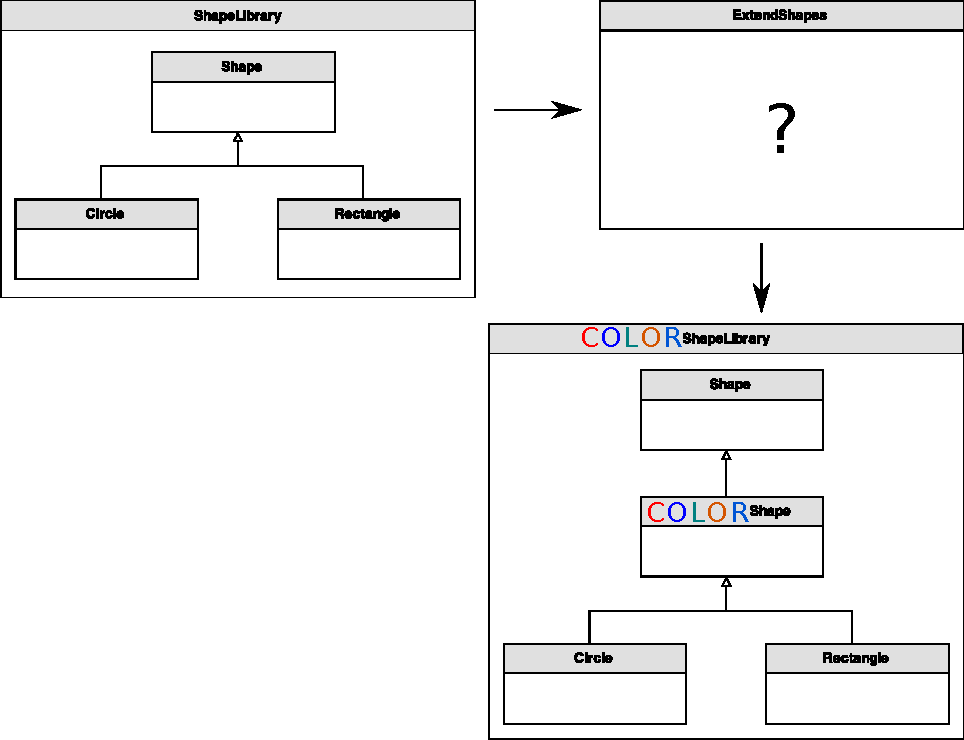
\includegraphics[width=0.8\textwidth]{resources/newspeak_inheritance_challenge.pdf}
\end{frame}

\begin{explainframe}{Example: Class Hierarchy Inheritance}
\begin{itemize}
  \item \lstinline{ShapeLibrary}: a library for geometrical shapes, containing classes \lstinline{Shape}, \lstinline{Circle}, \lstinline{Rectangle}
  \item \lstinline{Shape} is superclass of \lstinline{Circle} and \lstinline{Rectangle}, and provides basic rendering functionality
  \item \textbf{Challenge:} provide a module \lstinline{ExtendShapes} which takes as input $I$ any \lstinline{ShapeLibrary} and generates a modified \lstinline{ColorShapeLibrary} where \lstinline{ColorShapeLibrary.Shape} has additional behavior for drawing colors
  \begin{itemize}
    \item $I$ must have a nested class \lstinline{Shape}
    \item Override \lstinline{ColorShapeLibrary.Shape} with a new class whose superclass is $I$.\lstinline{Shape} (like method overriding)
  \end{itemize}
\end{itemize}
\end{explainframe}

\begin{frame}{Example: Class Hierarchy Inheritance in Newspeak \textsuperscript{[1]}}
\centering
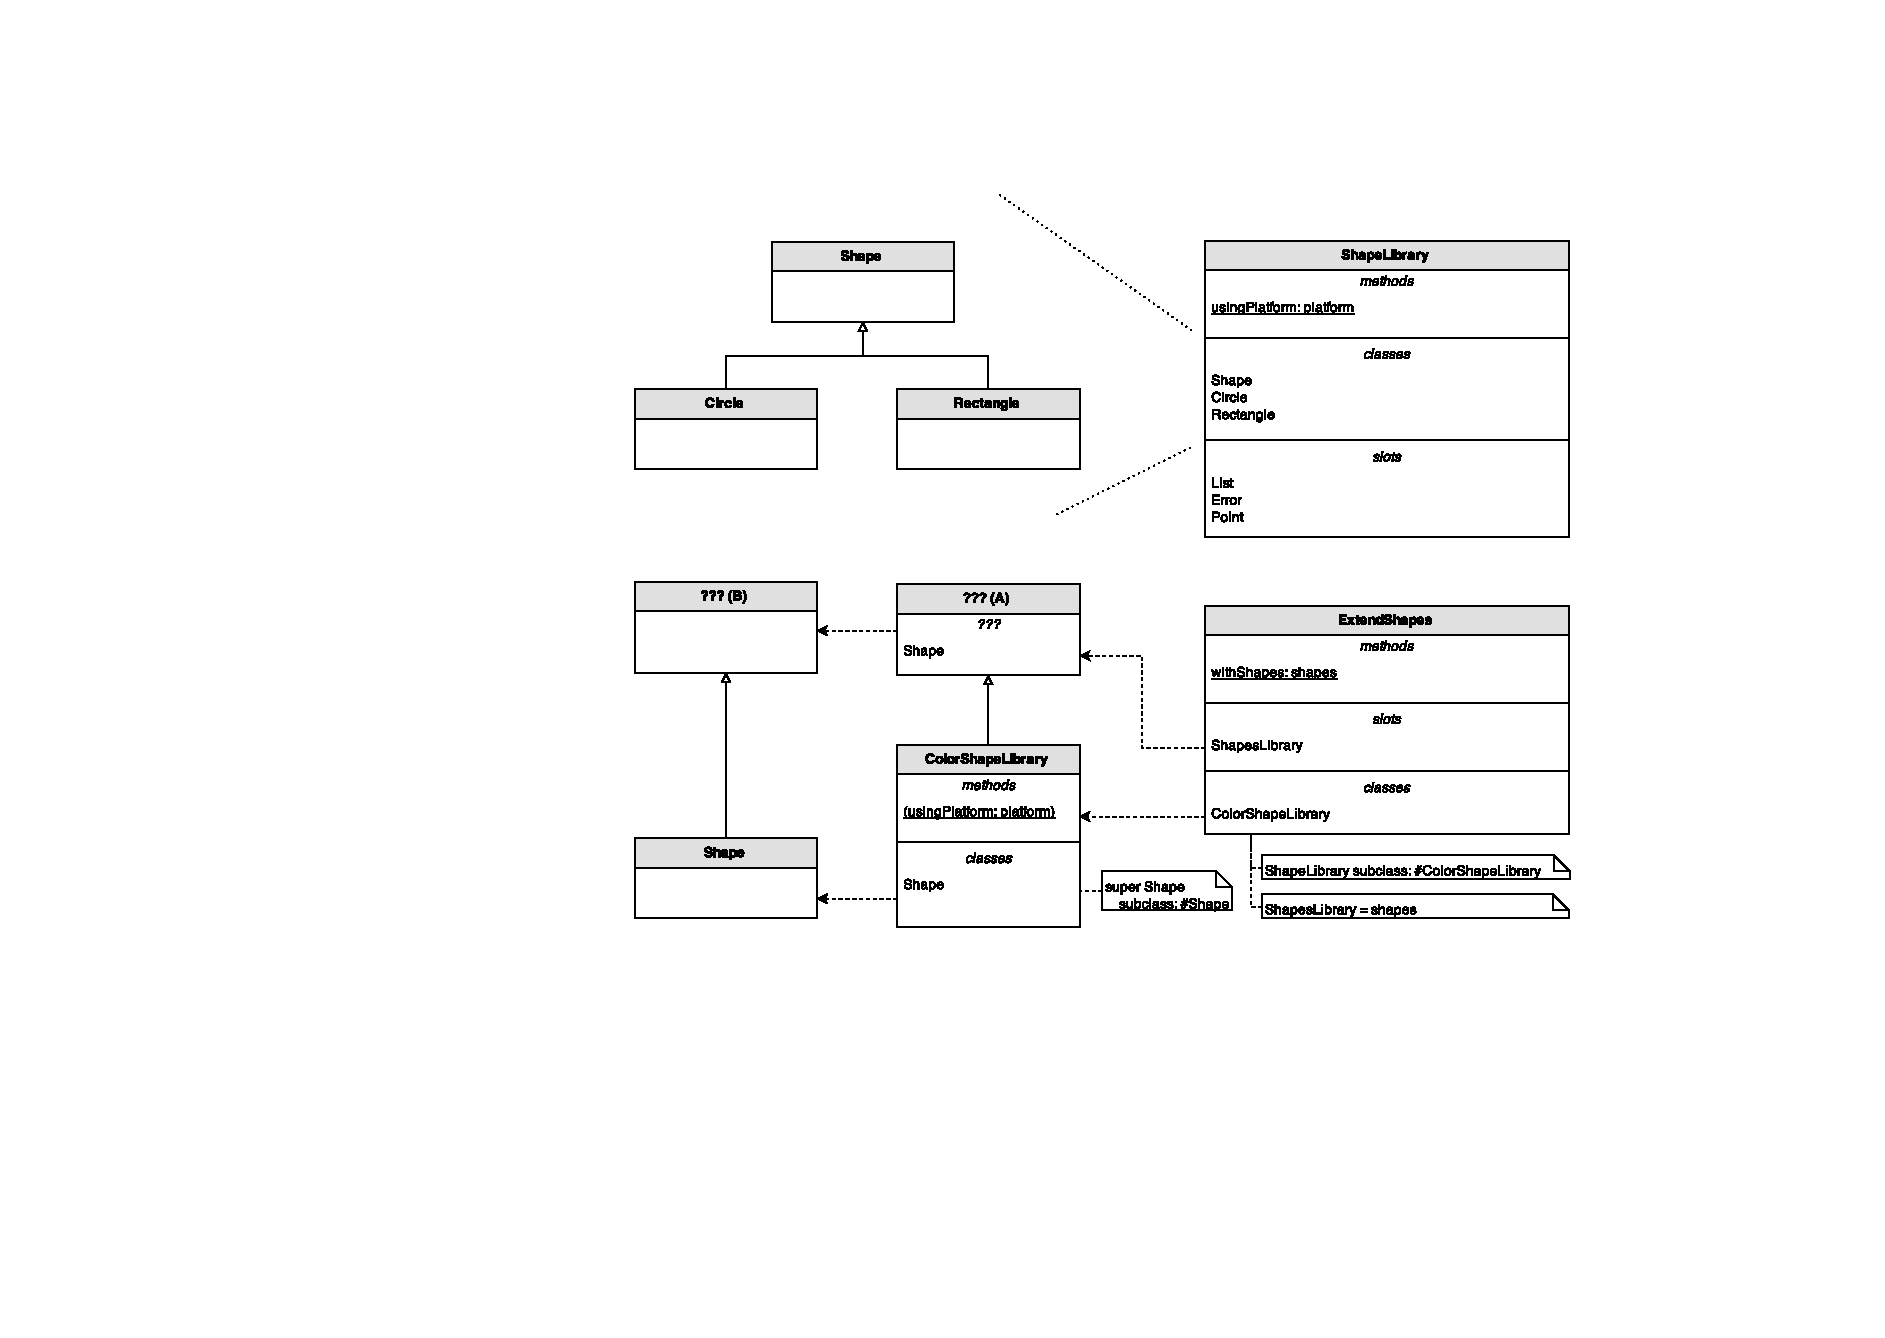
\includegraphics[width=0.8\textwidth]{resources/newspeak_inheritance}
\end{frame}

\begin{explainframe}{Class Hierarchy Inheritance $\rightarrow$ Smalltalk}
\begin{lstlisting}
Object sublcass: #ShapeLibrary
  instanceVariableNames: 'Shape Circle Rectangle List Error Point'.

ShapeLibrary>>Rectangle
  | nested | "nested is cached"
  nested := self Shape subclass: #Rectangle ...
  ... ^ nested

Object subclass: #ExtendShapes
  instanceVariableNames: 'ShapesLibrary ColorShapeLibrary'.

ExtendShapes class>>withShapes: shapes
  | inst | inst := self new.
  inst ShapesLibrary: shapes.
  ^ inst

ExtendedShapes>>ColorShapeLibrary
  | nested | "nested is cached"
  nested := self ShapesLibrary subclass: #ColorShapeLibrary instanceVariableNames: 'Shape'.
  nested class compile: 'usingPlatform: platform ^ ...'.
  nested compile: 'Shape | nested | "nested is cached" nested := super Shape subclass: #Shape. "add behavior to nested"'
  ^ nested
\end{lstlisting}
\end{explainframe}

\begin{explainframe}{Why Nested Classes are lazily initialized}
\begin{itemize}
  \item Consider nested classes are initialized in factory.
  \item \lstinline{ExtendedShape>>ColorShapeLibrary class>>usingPlatform:} triggers \lstinline{ShapeLibrary class>>usingPlatform:} (super constructor call).
  \item \lstinline{ShapeLibrary class>>usingPlatform:} creates \lstinline{Shape}, \lstinline{Circle}, \lstinline{Rectangle}.
  \item \lstinline{ExtendedShape>>ColorShapeLibrary class>>usingPlatform:} creates (overrides) a new \lstinline{Shape} class.
  \item \textbf{Problem:} \lstinline{Circle} and \lstinline{Rectangle} are still subclasses of the old \lstinline{Shape} class.
  \item \textbf{Solution:} all names are late bound and method calls. The method call \lstinline{Shape} creates the class on demand the superclass factory runs the subclass implementation (overridden).
\end{itemize}
\end{explainframe}

\begin{frame}{Method Lookup in Newspeak \textsuperscript{[1]}}
\centering
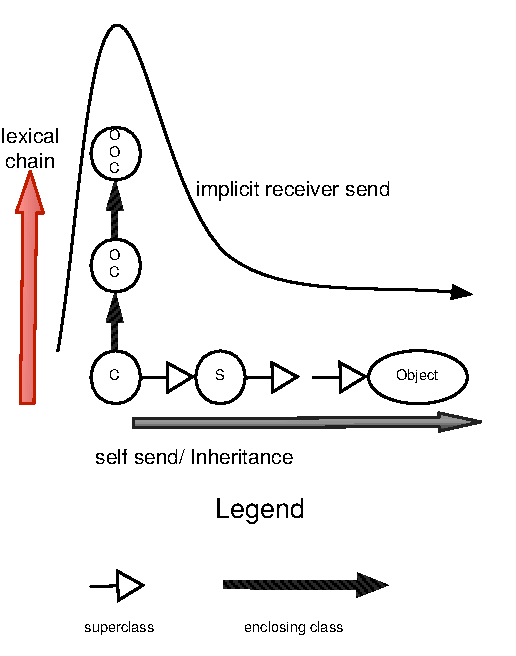
\includegraphics[width=0.5\textwidth]{resources/newspeak_lookup}
\end{frame}

\begin{explainframe}{Method Lookup in Newspeak}
\begin{itemize}
  \item First enclosing classes (\emph{lexical chain})
  \item Then superclass hierarchy
  \item Never check superclass hierarchy of enclosing classes
  \item Different from BETA and Java: \emph{comb semantics}
  \begin{itemize}
    \item Check receiver class and superclass hierarchy
    \item Check enclosing classes and superclass hierarchies
  \end{itemize}
\end{itemize}
\end{explainframe}

\begin{frame}[fragile]{Newspeak Avoids Method Name Clashes by Superclasses}{Example}
\begin{lstlisting}
class Super {
  //int m(){ return 42; }
}
class Outer {
  int m(){ return 91; }
  class Inner extends Super {
    int foo(){ return m(); }
  }
}
\end{lstlisting}

\lstinline{new Outer.Inner().foo()}?

\end{frame}

\begin{frame}{Poor Man's Nested Classes\textsuperscript{[4]}}{Classes as First Class Objects}
\begin{itemize}
  \item Scoping rules are different
  \item No convenient access to enclosing instance
  \item Hierarchy not reflected in the source code
  \item Bad tooling support
  \item No class hierarchy inheritance
\end{itemize}
\end{frame}

%\begin{frame}{Virtual Patterns}{Example (non-virtual)}
%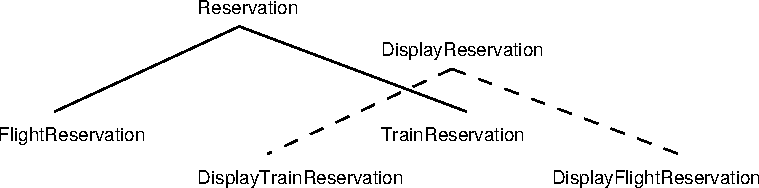
\includegraphics[width=\textwidth]{resources/beta_virtual}
%\vfill
%\begin{itemize}
%  \item \texttt{TrainReservation.DisplayTrainReservation} should be called \texttt{TrainReservation.DisplayReservation}
%  \item \texttt{FlightReservation.DisplayFlightReservation} should be called \texttt{FlightReservation.DisplayReservation}
%  \item \texttt{*.DisplayReservation} should be late bound and executed extended coded, not just base code
%\end{itemize}
%\end{frame}
%
%\begin{frame}[fragile]{Virtual Patterns}{Example}
%\begin{verbatim}
%Point:
%  (# X,Y: @integer;
%     Init:< (# do 0->X; 0->Y; inner #);
%  #)
%
%ThreeDPoint: Point
%  (# Z: @integer;
%     Init::< (# do 0->Z; inner #);
%  #)
%\end{verbatim}
%\end{frame}

\section{Summary}
\begin{frame}{Summary}
\begin{itemize}
  \item Pattern = Method = Class
  \item Nested patterns/classes: work like virtual methods in other programming languages
  \item More than Java nested classes: Java nested classes are not virtual
  \item Workaround for nested classes in other programming languages: factory
  \item No global namespace in Newspeak: \lstinline{platform} object provides all dependencies
  \item Newspeak: all names are late bound
\end{itemize}
\end{frame}

\begin{frame}{References}
\footnotesize
\begin{itemize}
  \item [1] Gilad Bracha, Peter Ahe, Vassili Bykov, Yaron Kashai, William Maddox and Eliot Miranda. Modules as Objects in Newspeak.
  \item [2] Gilad Bracha, Peter Ahe and Vassili Bykov. Newspeak on Squeak: A Guide for the Perplexed.
  \item [3] Gilad Bracha, Peter Ahe, Vassili Bykov, Yaron Kashai and Eliot Miranda. The Newspeak Programming Platform. 
  \item [4] \url{http://gbracha.blogspot.jp/2013/01/inheriting-class.html}
  \item [5] \url{http://www.cs.au.dk/~beta/Manuals/r5.2.2/beta-intro/Virtual.html}
  \item [6] Bent Bruun Kristensen, Ole Lehrmann Madsen, and Birger Møller-Pedersen. 2007. The when, why and why not of the BETA programming language.
  \item [7]  Madsen, O. L.: Abstraction and Modularization in the BETA Programming Language.
  \item [8] \url{http://gbracha.blogspot.de/2008/12/living-without-global-namespaces.html}
\end{itemize}
\end{frame}
\end{document}
